\documentclass[1p]{elsarticle_modified}
%\bibliographystyle{elsarticle-num}

%\usepackage[colorlinks]{hyperref}
%\usepackage{abbrmath_seonhwa} %\Abb, \Ascr, \Acal ,\Abf, \Afrak
\usepackage{amsfonts}
\usepackage{amssymb}
\usepackage{amsmath}
\usepackage{amsthm}
\usepackage{scalefnt}
\usepackage{amsbsy}
\usepackage{kotex}
\usepackage{caption}
\usepackage{subfig}
\usepackage{color}
\usepackage{graphicx}
\usepackage{xcolor} %% white, black, red, green, blue, cyan, magenta, yellow
\usepackage{float}
\usepackage{setspace}
\usepackage{hyperref}

\usepackage{tikz}
\usetikzlibrary{arrows}

\usepackage{multirow}
\usepackage{array} % fixed length table
\usepackage{hhline}

%%%%%%%%%%%%%%%%%%%%%
\makeatletter
\renewcommand*\env@matrix[1][\arraystretch]{%
	\edef\arraystretch{#1}%
	\hskip -\arraycolsep
	\let\@ifnextchar\new@ifnextchar
	\array{*\c@MaxMatrixCols c}}
\makeatother %https://tex.stackexchange.com/questions/14071/how-can-i-increase-the-line-spacing-in-a-matrix
%%%%%%%%%%%%%%%

\usepackage[normalem]{ulem}

\newcommand{\msout}[1]{\ifmmode\text{\sout{\ensuremath{#1}}}\else\sout{#1}\fi}
%SOURCE: \msout is \stkout macro in https://tex.stackexchange.com/questions/20609/strikeout-in-math-mode

\newcommand{\cancel}[1]{
	\ifmmode
	{\color{red}\msout{#1}}
	\else
	{\color{red}\sout{#1}}
	\fi
}

\newcommand{\add}[1]{
	{\color{blue}\uwave{#1}}
}

\newcommand{\replace}[2]{
	\ifmmode
	{\color{red}\msout{#1}}{\color{blue}\uwave{#2}}
	\else
	{\color{red}\sout{#1}}{\color{blue}\uwave{#2}}
	\fi
}

\newcommand{\Sol}{\mathcal{S}} %segment
\newcommand{\D}{D} %diagram
\newcommand{\A}{\mathcal{A}} %arc


%%%%%%%%%%%%%%%%%%%%%%%%%%%%%5 test

\def\sl{\operatorname{\textup{SL}}(2,\Cbb)}
\def\psl{\operatorname{\textup{PSL}}(2,\Cbb)}
\def\quan{\mkern 1mu \triangleright \mkern 1mu}

\theoremstyle{definition}
\newtheorem{thm}{Theorem}[section]
\newtheorem{prop}[thm]{Proposition}
\newtheorem{lem}[thm]{Lemma}
\newtheorem{ques}[thm]{Question}
\newtheorem{cor}[thm]{Corollary}
\newtheorem{defn}[thm]{Definition}
\newtheorem{exam}[thm]{Example}
\newtheorem{rmk}[thm]{Remark}
\newtheorem{alg}[thm]{Algorithm}

\newcommand{\I}{\sqrt{-1}}
\begin{document}

%\begin{frontmatter}
%
%\title{Boundary parabolic representations of knots up to 8 crossings}
%
%%% Group authors per affiliation:
%\author{Yunhi Cho} 
%\address{Department of Mathematics, University of Seoul, Seoul, Korea}
%\ead{yhcho@uos.ac.kr}
%
%
%\author{Seonhwa Kim} %\fnref{s_kim}}
%\address{Center for Geometry and Physics, Institute for Basic Science, Pohang, 37673, Korea}
%\ead{ryeona17@ibs.re.kr}
%
%\author{Hyuk Kim}
%\address{Department of Mathematical Sciences, Seoul National University, Seoul 08826, Korea}
%\ead{hyukkim@snu.ac.kr}
%
%\author{Seokbeom Yoon}
%\address{Department of Mathematical Sciences, Seoul National University, Seoul, 08826,  Korea}
%\ead{sbyoon15@snu.ac.kr}
%
%\begin{abstract}
%We find all boundary parabolic representation of knots up to 8 crossings.
%
%\end{abstract}
%\begin{keyword}
%    \MSC[2010] 57M25 
%\end{keyword}
%
%\end{frontmatter}

%\linenumbers
%\tableofcontents
%
\newcommand\colored[1]{\textcolor{white}{\rule[-0.35ex]{0.8em}{1.4ex}}\kern-0.8em\color{red} #1}%
%\newcommand\colored[1]{\textcolor{white}{ #1}\kern-2.17ex	\textcolor{white}{ #1}\kern-1.81ex	\textcolor{white}{ #1}\kern-2.15ex\color{red}#1	}

{\Large $\underline{12a_{0238}~(K12a_{0238})}$}

\setlength{\tabcolsep}{10pt}
\renewcommand{\arraystretch}{1.6}
\vspace{1cm}\begin{tabular}{m{100pt}>{\centering\arraybackslash}m{274pt}}
\multirow{5}{120pt}{
	\centering
	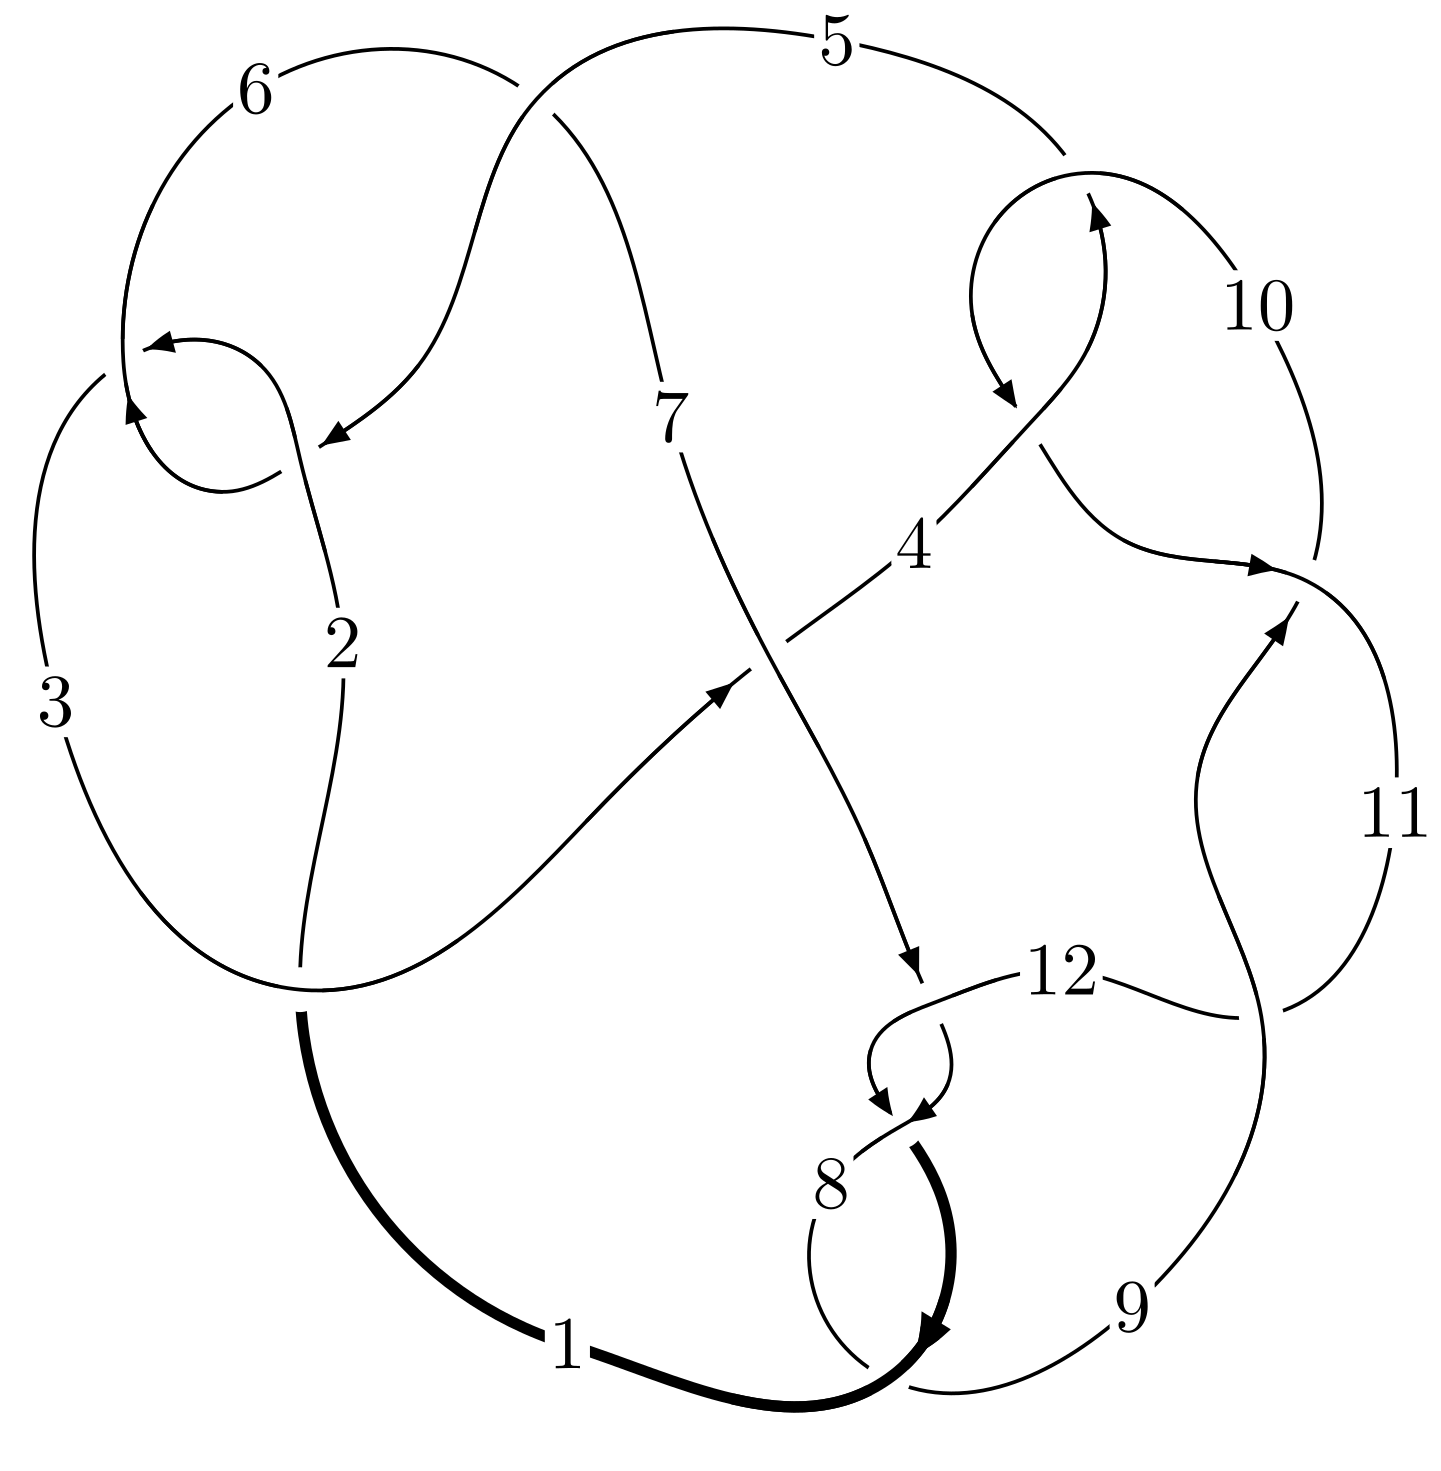
\includegraphics[width=112pt]{../../../GIT/diagram.site/Diagrams/png/1039_12a_0238.png}\\
\ \ \ A knot diagram\footnotemark}&
\allowdisplaybreaks
\textbf{Linearized knot diagam} \\
\cline{2-2}
 &
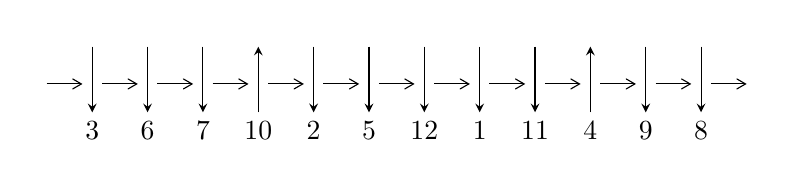
\begin{tikzpicture}[x=20pt, y=17pt]
	% nodes
	\node (C0) at (0, 0) {};
	\node (C1) at (1, 0) {};
	\node (C1U) at (1, +1) {};
	\node (C1D) at (1, -1) {3};

	\node (C2) at (2, 0) {};
	\node (C2U) at (2, +1) {};
	\node (C2D) at (2, -1) {6};

	\node (C3) at (3, 0) {};
	\node (C3U) at (3, +1) {};
	\node (C3D) at (3, -1) {7};

	\node (C4) at (4, 0) {};
	\node (C4U) at (4, +1) {};
	\node (C4D) at (4, -1) {10};

	\node (C5) at (5, 0) {};
	\node (C5U) at (5, +1) {};
	\node (C5D) at (5, -1) {2};

	\node (C6) at (6, 0) {};
	\node (C6U) at (6, +1) {};
	\node (C6D) at (6, -1) {5};

	\node (C7) at (7, 0) {};
	\node (C7U) at (7, +1) {};
	\node (C7D) at (7, -1) {12};

	\node (C8) at (8, 0) {};
	\node (C8U) at (8, +1) {};
	\node (C8D) at (8, -1) {1};

	\node (C9) at (9, 0) {};
	\node (C9U) at (9, +1) {};
	\node (C9D) at (9, -1) {11};

	\node (C10) at (10, 0) {};
	\node (C10U) at (10, +1) {};
	\node (C10D) at (10, -1) {4};

	\node (C11) at (11, 0) {};
	\node (C11U) at (11, +1) {};
	\node (C11D) at (11, -1) {9};

	\node (C12) at (12, 0) {};
	\node (C12U) at (12, +1) {};
	\node (C12D) at (12, -1) {8};
	\node (C13) at (13, 0) {};

	% arrows
	\draw[->,>={angle 60}]
	(C0) edge (C1) (C1) edge (C2) (C2) edge (C3) (C3) edge (C4) (C4) edge (C5) (C5) edge (C6) (C6) edge (C7) (C7) edge (C8) (C8) edge (C9) (C9) edge (C10) (C10) edge (C11) (C11) edge (C12) (C12) edge (C13) ;	\draw[->,>=stealth]
	(C1U) edge (C1D) (C2U) edge (C2D) (C3U) edge (C3D) (C4D) edge (C4U) (C5U) edge (C5D) (C6U) edge (C6D) (C7U) edge (C7D) (C8U) edge (C8D) (C9U) edge (C9D) (C10D) edge (C10U) (C11U) edge (C11D) (C12U) edge (C12D) ;
	\end{tikzpicture} \\
\hhline{~~} \\& 
\textbf{Solving Sequence} \\ \cline{2-2} 
 &
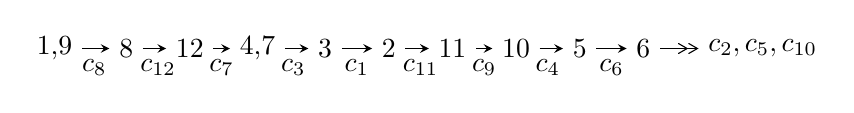
\begin{tikzpicture}[x=23pt, y=7pt]
	% node
	\node (A0) at (-1/8, 0) {1,9};
	\node (A1) at (1, 0) {8};
	\node (A2) at (2, 0) {12};
	\node (A3) at (49/16, 0) {4,7};
	\node (A4) at (33/8, 0) {3};
	\node (A5) at (41/8, 0) {2};
	\node (A6) at (49/8, 0) {11};
	\node (A7) at (57/8, 0) {10};
	\node (A8) at (65/8, 0) {5};
	\node (A9) at (73/8, 0) {6};
	\node (C1) at (1/2, -1) {$c_{8}$};
	\node (C2) at (3/2, -1) {$c_{12}$};
	\node (C3) at (5/2, -1) {$c_{7}$};
	\node (C4) at (29/8, -1) {$c_{3}$};
	\node (C5) at (37/8, -1) {$c_{1}$};
	\node (C6) at (45/8, -1) {$c_{11}$};
	\node (C7) at (53/8, -1) {$c_{9}$};
	\node (C8) at (61/8, -1) {$c_{4}$};
	\node (C9) at (69/8, -1) {$c_{6}$};
	\node (A10) at (11, 0) {$c_{2},c_{5},c_{10}$};

	% edge
	\draw[->,>=stealth]	
	(A0) edge (A1) (A1) edge (A2) (A2) edge (A3) (A3) edge (A4) (A4) edge (A5) (A5) edge (A6) (A6) edge (A7) (A7) edge (A8) (A8) edge (A9) ;
	\draw[->>,>={angle 60}]	
	(A9) edge (A10);
\end{tikzpicture} \\ 

\end{tabular} \\

\footnotetext{
The image of knot diagram is generated by the software ``\textbf{Draw programme}" developed by Andrew Bartholomew(\url{http://www.layer8.co.uk/maths/draw/index.htm\#Running-draw}), where we modified some parts for our purpose(\url{https://github.com/CATsTAILs/LinksPainter}).
}\phantom \\ \newline 
\centering \textbf{Ideals for irreducible components\footnotemark of $X_{\text{par}}$} 
 
\begin{align*}
I^u_{1}&=\langle 
u^{76}- u^{75}+\cdots+2 b-1,\;97 u^{76}+269 u^{75}+\cdots+4 a+83,\;u^{77}+4 u^{76}+\cdots+2 u+1\rangle \\
I^u_{2}&=\langle 
b,\;a^3+a^2+2 a+1,\;u-1\rangle \\
\\
\end{align*}
\raggedright * 2 irreducible components of $\dim_{\mathbb{C}}=0$, with total 80 representations.\\
\footnotetext{All coefficients of polynomials are rational numbers. But the coefficients are sometimes approximated in decimal forms when there is not enough margin.}
\newpage
\renewcommand{\arraystretch}{1}
\centering \section*{I. $I^u_{1}= \langle u^{76}- u^{75}+\cdots+2 b-1,\;97 u^{76}+269 u^{75}+\cdots+4 a+83,\;u^{77}+4 u^{76}+\cdots+2 u+1 \rangle$}
\flushleft \textbf{(i) Arc colorings}\\
\begin{tabular}{m{7pt} m{180pt} m{7pt} m{180pt} }
\flushright $a_{1}=$&$\begin{pmatrix}0\\u\end{pmatrix}$ \\
\flushright $a_{9}=$&$\begin{pmatrix}1\\0\end{pmatrix}$ \\
\flushright $a_{8}=$&$\begin{pmatrix}1\\- u^2\end{pmatrix}$ \\
\flushright $a_{12}=$&$\begin{pmatrix}u\\- u^3+u\end{pmatrix}$ \\
\flushright $a_{4}=$&$\begin{pmatrix}-24.2500 u^{76}-67.2500 u^{75}+\cdots-17.2500 u-20.7500\\-\frac{1}{2} u^{76}+\frac{1}{2} u^{75}+\cdots+\frac{1}{2} u+\frac{1}{2}\end{pmatrix}$ \\
\flushright $a_{7}=$&$\begin{pmatrix}- u^2+1\\u^4-2 u^2\end{pmatrix}$ \\
\flushright $a_{3}=$&$\begin{pmatrix}-16.2500 u^{76}-45.2500 u^{75}+\cdots-9.25000 u-14.7500\\\frac{43}{4} u^{76}+\frac{123}{4} u^{75}+\cdots+\frac{43}{4} u+\frac{37}{4}\end{pmatrix}$ \\
\flushright $a_{2}=$&$\begin{pmatrix}\frac{1}{4} u^{76}+\frac{3}{4} u^{75}+\cdots-\frac{23}{4} u+\frac{5}{4}\\-\frac{1}{4} u^{76}-\frac{3}{4} u^{75}+\cdots-\frac{1}{4} u-\frac{1}{4}\end{pmatrix}$ \\
\flushright $a_{11}=$&$\begin{pmatrix}- u^3+2 u\\- u^3+u\end{pmatrix}$ \\
\flushright $a_{10}=$&$\begin{pmatrix}u^6-3 u^4+2 u^2+1\\u^6-2 u^4+u^2\end{pmatrix}$ \\
\flushright $a_{5}=$&$\begin{pmatrix}-12.7500 u^{76}-35.7500 u^{75}+\cdots-4.75000 u-11.2500\\\frac{33}{2} u^{76}+\frac{89}{2} u^{75}+\cdots+\frac{33}{2} u+\frac{25}{2}\end{pmatrix}$ \\
\flushright $a_{6}=$&$\begin{pmatrix}-\frac{1}{4} u^{76}-\frac{3}{4} u^{75}+\cdots+\frac{23}{4} u-\frac{1}{4}\\u^{19}-7 u^{17}+\cdots-6 u^2+u\end{pmatrix}$\\&\end{tabular}
\flushleft \textbf{(ii) Obstruction class $= -1$}\\~\\
\flushleft \textbf{(iii) Cusp Shapes $= 42 u^{76}+\frac{231}{2} u^{75}+\cdots+43 u+\frac{53}{2}$}\\~\\
\newpage\renewcommand{\arraystretch}{1}
\flushleft \textbf{(iv) u-Polynomials at the component}\newline \\
\begin{tabular}{m{50pt}|m{274pt}}
Crossings & \hspace{64pt}u-Polynomials at each crossing \\
\hline $$\begin{aligned}c_{1},c_{6}\end{aligned}$$&$\begin{aligned}
&u^{77}+24 u^{76}+\cdots+13 u+1
\end{aligned}$\\
\hline $$\begin{aligned}c_{2},c_{5}\end{aligned}$$&$\begin{aligned}
&u^{77}+2 u^{76}+\cdots-3 u-1
\end{aligned}$\\
\hline $$\begin{aligned}c_{3}\end{aligned}$$&$\begin{aligned}
&u^{77}-2 u^{76}+\cdots+15757 u-4753
\end{aligned}$\\
\hline $$\begin{aligned}c_{4},c_{10}\end{aligned}$$&$\begin{aligned}
&u^{77}+u^{76}+\cdots-36 u-8
\end{aligned}$\\
\hline $$\begin{aligned}c_{7},c_{8},c_{12}\end{aligned}$$&$\begin{aligned}
&u^{77}-4 u^{76}+\cdots+2 u-1
\end{aligned}$\\
\hline $$\begin{aligned}c_{9},c_{11}\end{aligned}$$&$\begin{aligned}
&u^{77}+21 u^{76}+\cdots-432 u-64
\end{aligned}$\\
\hline
\end{tabular}\\~\\
\newpage\renewcommand{\arraystretch}{1}
\flushleft \textbf{(v) Riley Polynomials at the component}\newline \\
\begin{tabular}{m{50pt}|m{274pt}}
Crossings & \hspace{64pt}Riley Polynomials at each crossing \\
\hline $$\begin{aligned}c_{1},c_{6}\end{aligned}$$&$\begin{aligned}
&y^{77}+60 y^{76}+\cdots+61 y-1
\end{aligned}$\\
\hline $$\begin{aligned}c_{2},c_{5}\end{aligned}$$&$\begin{aligned}
&y^{77}-24 y^{76}+\cdots+13 y-1
\end{aligned}$\\
\hline $$\begin{aligned}c_{3}\end{aligned}$$&$\begin{aligned}
&y^{77}+24 y^{76}+\cdots+306820997 y-22591009
\end{aligned}$\\
\hline $$\begin{aligned}c_{4},c_{10}\end{aligned}$$&$\begin{aligned}
&y^{77}+21 y^{76}+\cdots-432 y-64
\end{aligned}$\\
\hline $$\begin{aligned}c_{7},c_{8},c_{12}\end{aligned}$$&$\begin{aligned}
&y^{77}-62 y^{76}+\cdots+26 y-1
\end{aligned}$\\
\hline $$\begin{aligned}c_{9},c_{11}\end{aligned}$$&$\begin{aligned}
&y^{77}+65 y^{76}+\cdots+232704 y-4096
\end{aligned}$\\
\hline
\end{tabular}\\~\\
\newpage\flushleft \textbf{(vi) Complex Volumes and Cusp Shapes}
$$\begin{array}{c|c|c}  
\text{Solutions to }I^u_{1}& \I (\text{vol} + \sqrt{-1}CS) & \text{Cusp shape}\\
 \hline 
\begin{aligned}
u &= \phantom{-}1.10650\phantom{ +0.000000I} \\
a &= \phantom{-}0.143141\phantom{ +0.000000I} \\
b &= -0.621888\phantom{ +0.000000I}\end{aligned}
 & -2.08407\phantom{ +0.000000I} & \phantom{-0.000000 } 0 \\ \hline\begin{aligned}
u &= \phantom{-}0.097508 + 0.886073 I \\
a &= -0.93635 - 2.39335 I \\
b &= -0.98803 - 1.89695 I\end{aligned}
 & \phantom{-}7.58861 - 11.05880 I & \phantom{-0.000000 } 0 \\ \hline\begin{aligned}
u &= \phantom{-}0.097508 - 0.886073 I \\
a &= -0.93635 + 2.39335 I \\
b &= -0.98803 + 1.89695 I\end{aligned}
 & \phantom{-}7.58861 + 11.05880 I & \phantom{-0.000000 } 0 \\ \hline\begin{aligned}
u &= \phantom{-}0.084767 + 0.881704 I \\
a &= \phantom{-}0.82424 + 2.45291 I \\
b &= \phantom{-}0.91399 + 1.93588 I\end{aligned}
 & \phantom{-}8.41612 - 5.12553 I & \phantom{-0.000000 } 0 \\ \hline\begin{aligned}
u &= \phantom{-}0.084767 - 0.881704 I \\
a &= \phantom{-}0.82424 - 2.45291 I \\
b &= \phantom{-}0.91399 - 1.93588 I\end{aligned}
 & \phantom{-}8.41612 + 5.12553 I & \phantom{-0.000000 } 0 \\ \hline\begin{aligned}
u &= \phantom{-}0.808057 + 0.354660 I \\
a &= \phantom{-}0.398327 + 0.653038 I \\
b &= \phantom{-}0.154983 - 0.382042 I\end{aligned}
 & -0.06970 - 2.22982 I & \phantom{-0.000000 } 0 \\ \hline\begin{aligned}
u &= \phantom{-}0.808057 - 0.354660 I \\
a &= \phantom{-}0.398327 - 0.653038 I \\
b &= \phantom{-}0.154983 + 0.382042 I\end{aligned}
 & -0.06970 + 2.22982 I & \phantom{-0.000000 } 0 \\ \hline\begin{aligned}
u &= \phantom{-}0.105277 + 0.833083 I \\
a &= -0.63268 - 2.02197 I \\
b &= -0.79075 - 1.65686 I\end{aligned}
 & \phantom{-}1.48971 - 5.79921 I & -8.00000 + 6.61448 I \\ \hline\begin{aligned}
u &= \phantom{-}0.105277 - 0.833083 I \\
a &= -0.63268 + 2.02197 I \\
b &= -0.79075 + 1.65686 I\end{aligned}
 & \phantom{-}1.48971 + 5.79921 I & -8.00000 - 6.61448 I \\ \hline\begin{aligned}
u &= -0.017153 + 0.834554 I \\
a &= -0.16213 + 2.72359 I \\
b &= \phantom{-}0.26575 + 2.08207 I\end{aligned}
 & \phantom{-}8.84895 - 1.05261 I & -1.57002 + 2.20450 I\\
 \hline 
 \end{array}$$\newpage$$\begin{array}{c|c|c}  
\text{Solutions to }I^u_{1}& \I (\text{vol} + \sqrt{-1}CS) & \text{Cusp shape}\\
 \hline 
\begin{aligned}
u &= -0.017153 - 0.834554 I \\
a &= -0.16213 - 2.72359 I \\
b &= \phantom{-}0.26575 - 2.08207 I\end{aligned}
 & \phantom{-}8.84895 + 1.05261 I & -1.57002 - 2.20450 I \\ \hline\begin{aligned}
u &= \phantom{-}0.055315 + 0.827179 I \\
a &= \phantom{-}0.29493 + 2.28516 I \\
b &= \phantom{-}0.57429 + 1.82055 I\end{aligned}
 & \phantom{-}4.87219 - 2.94616 I & -1.74736 + 3.05981 I \\ \hline\begin{aligned}
u &= \phantom{-}0.055315 - 0.827179 I \\
a &= \phantom{-}0.29493 - 2.28516 I \\
b &= \phantom{-}0.57429 - 1.82055 I\end{aligned}
 & \phantom{-}4.87219 + 2.94616 I & -1.74736 - 3.05981 I \\ \hline\begin{aligned}
u &= -0.032046 + 0.825605 I \\
a &= \phantom{-}0.31484 - 2.72986 I \\
b &= -0.16740 - 2.07689 I\end{aligned}
 & \phantom{-}8.13865 + 4.89439 I & -2.77959 - 2.93491 I \\ \hline\begin{aligned}
u &= -0.032046 - 0.825605 I \\
a &= \phantom{-}0.31484 + 2.72986 I \\
b &= -0.16740 + 2.07689 I\end{aligned}
 & \phantom{-}8.13865 - 4.89439 I & -2.77959 + 2.93491 I \\ \hline\begin{aligned}
u &= \phantom{-}0.708066 + 0.417899 I \\
a &= -0.248020 - 0.776113 I \\
b &= -0.095443 + 0.246952 I\end{aligned}
 & -0.36212 + 2.86972 I & -12.09253 - 2.69400 I \\ \hline\begin{aligned}
u &= \phantom{-}0.708066 - 0.417899 I \\
a &= -0.248020 + 0.776113 I \\
b &= -0.095443 - 0.246952 I\end{aligned}
 & -0.36212 - 2.86972 I & -12.09253 + 2.69400 I \\ \hline\begin{aligned}
u &= -1.191750 + 0.014551 I \\
a &= -0.15908 + 1.89115 I \\
b &= \phantom{-}0.016839 - 0.355506 I\end{aligned}
 & \phantom{-}0.50247 + 2.96603 I & \phantom{-0.000000 } 0 \\ \hline\begin{aligned}
u &= -1.191750 - 0.014551 I \\
a &= -0.15908 - 1.89115 I \\
b &= \phantom{-}0.016839 + 0.355506 I\end{aligned}
 & \phantom{-}0.50247 - 2.96603 I & \phantom{-0.000000 } 0 \\ \hline\begin{aligned}
u &= \phantom{-}1.143870 + 0.381225 I \\
a &= \phantom{-}1.095240 - 0.097934 I \\
b &= \phantom{-}0.245777 - 1.386210 I\end{aligned}
 & -1.69396 + 1.41527 I & \phantom{-0.000000 } 0\\
 \hline 
 \end{array}$$\newpage$$\begin{array}{c|c|c}  
\text{Solutions to }I^u_{1}& \I (\text{vol} + \sqrt{-1}CS) & \text{Cusp shape}\\
 \hline 
\begin{aligned}
u &= \phantom{-}1.143870 - 0.381225 I \\
a &= \phantom{-}1.095240 + 0.097934 I \\
b &= \phantom{-}0.245777 + 1.386210 I\end{aligned}
 & -1.69396 - 1.41527 I & \phantom{-0.000000 } 0 \\ \hline\begin{aligned}
u &= \phantom{-}0.027991 + 0.770737 I \\
a &= \phantom{-}0.17046 - 2.07494 I \\
b &= -0.29207 - 1.67629 I\end{aligned}
 & \phantom{-}1.86989 + 0.11087 I & -7.62813 - 0.98718 I \\ \hline\begin{aligned}
u &= \phantom{-}0.027991 - 0.770737 I \\
a &= \phantom{-}0.17046 + 2.07494 I \\
b &= -0.29207 + 1.67629 I\end{aligned}
 & \phantom{-}1.86989 - 0.11087 I & -7.62813 + 0.98718 I \\ \hline\begin{aligned}
u &= \phantom{-}1.252950 + 0.126715 I \\
a &= \phantom{-}0.063260 - 0.352922 I \\
b &= -1.28347 - 0.85286 I\end{aligned}
 & -1.123090 + 0.200004 I & \phantom{-0.000000 } 0 \\ \hline\begin{aligned}
u &= \phantom{-}1.252950 - 0.126715 I \\
a &= \phantom{-}0.063260 + 0.352922 I \\
b &= -1.28347 + 0.85286 I\end{aligned}
 & -1.123090 - 0.200004 I & \phantom{-0.000000 } 0 \\ \hline\begin{aligned}
u &= \phantom{-}1.181210 + 0.451223 I \\
a &= \phantom{-}1.52706 - 0.14826 I \\
b &= \phantom{-}0.65607 - 1.67635 I\end{aligned}
 & \phantom{-}4.26251 + 6.28683 I & \phantom{-0.000000 } 0 \\ \hline\begin{aligned}
u &= \phantom{-}1.181210 - 0.451223 I \\
a &= \phantom{-}1.52706 + 0.14826 I \\
b &= \phantom{-}0.65607 + 1.67635 I\end{aligned}
 & \phantom{-}4.26251 - 6.28683 I & \phantom{-0.000000 } 0 \\ \hline\begin{aligned}
u &= \phantom{-}0.384694 + 0.626756 I \\
a &= \phantom{-}0.401391 - 0.155030 I \\
b &= \phantom{-}0.489003 + 0.393854 I\end{aligned}
 & \phantom{-}0.62637 - 6.82755 I & -8.78463 + 9.37129 I \\ \hline\begin{aligned}
u &= \phantom{-}0.384694 - 0.626756 I \\
a &= \phantom{-}0.401391 + 0.155030 I \\
b &= \phantom{-}0.489003 - 0.393854 I\end{aligned}
 & \phantom{-}0.62637 + 6.82755 I & -8.78463 - 9.37129 I \\ \hline\begin{aligned}
u &= \phantom{-}1.194370 + 0.441307 I \\
a &= -1.50076 + 0.24788 I \\
b &= -0.57839 + 1.76571 I\end{aligned}
 & \phantom{-}5.00644 + 0.39923 I & \phantom{-0.000000 } 0\\
 \hline 
 \end{array}$$\newpage$$\begin{array}{c|c|c}  
\text{Solutions to }I^u_{1}& \I (\text{vol} + \sqrt{-1}CS) & \text{Cusp shape}\\
 \hline 
\begin{aligned}
u &= \phantom{-}1.194370 - 0.441307 I \\
a &= -1.50076 - 0.24788 I \\
b &= -0.57839 - 1.76571 I\end{aligned}
 & \phantom{-}5.00644 - 0.39923 I & \phantom{-0.000000 } 0 \\ \hline\begin{aligned}
u &= \phantom{-}1.218780 + 0.371520 I \\
a &= -1.131810 + 0.490210 I \\
b &= -0.05039 + 1.82641 I\end{aligned}
 & \phantom{-}1.29259 - 1.36850 I & \phantom{-0.000000 } 0 \\ \hline\begin{aligned}
u &= \phantom{-}1.218780 - 0.371520 I \\
a &= -1.131810 - 0.490210 I \\
b &= -0.05039 - 1.82641 I\end{aligned}
 & \phantom{-}1.29259 + 1.36850 I & \phantom{-0.000000 } 0 \\ \hline\begin{aligned}
u &= \phantom{-}1.27596\phantom{ +0.000000I} \\
a &= \phantom{-}0.162112\phantom{ +0.000000I} \\
b &= \phantom{-}1.61262\phantom{ +0.000000I}\end{aligned}
 & -5.58576\phantom{ +0.000000I} & \phantom{-0.000000 } 0 \\ \hline\begin{aligned}
u &= \phantom{-}1.289500 + 0.093349 I \\
a &= \phantom{-}0.118640 + 0.332675 I \\
b &= \phantom{-}1.61535 + 0.70924 I\end{aligned}
 & -1.70313 - 4.94998 I & \phantom{-0.000000 } 0 \\ \hline\begin{aligned}
u &= \phantom{-}1.289500 - 0.093349 I \\
a &= \phantom{-}0.118640 - 0.332675 I \\
b &= \phantom{-}1.61535 - 0.70924 I\end{aligned}
 & -1.70313 + 4.94998 I & \phantom{-0.000000 } 0 \\ \hline\begin{aligned}
u &= -1.242140 + 0.370004 I \\
a &= -1.83348 - 0.78636 I \\
b &= \phantom{-}0.47585 - 1.69036 I\end{aligned}
 & \phantom{-}4.40113 - 0.59472 I & \phantom{-0.000000 } 0 \\ \hline\begin{aligned}
u &= -1.242140 - 0.370004 I \\
a &= -1.83348 + 0.78636 I \\
b &= \phantom{-}0.47585 + 1.69036 I\end{aligned}
 & \phantom{-}4.40113 + 0.59472 I & \phantom{-0.000000 } 0 \\ \hline\begin{aligned}
u &= \phantom{-}0.486786 + 0.502721 I \\
a &= \phantom{-}0.054759 - 0.547642 I \\
b &= \phantom{-}0.197801 + 0.269349 I\end{aligned}
 & -3.72778 - 1.85875 I & -16.4618 + 5.2268 I \\ \hline\begin{aligned}
u &= \phantom{-}0.486786 - 0.502721 I \\
a &= \phantom{-}0.054759 + 0.547642 I \\
b &= \phantom{-}0.197801 - 0.269349 I\end{aligned}
 & -3.72778 + 1.85875 I & -16.4618 - 5.2268 I\\
 \hline 
 \end{array}$$\newpage$$\begin{array}{c|c|c}  
\text{Solutions to }I^u_{1}& \I (\text{vol} + \sqrt{-1}CS) & \text{Cusp shape}\\
 \hline 
\begin{aligned}
u &= \phantom{-}1.257860 + 0.329615 I \\
a &= \phantom{-}0.896116 - 0.718720 I \\
b &= -0.35639 - 1.95698 I\end{aligned}
 & -1.93916 - 4.07565 I & \phantom{-0.000000 } 0 \\ \hline\begin{aligned}
u &= \phantom{-}1.257860 - 0.329615 I \\
a &= \phantom{-}0.896116 + 0.718720 I \\
b &= -0.35639 + 1.95698 I\end{aligned}
 & -1.93916 + 4.07565 I & \phantom{-0.000000 } 0 \\ \hline\begin{aligned}
u &= -1.255060 + 0.377694 I \\
a &= \phantom{-}1.75729 + 0.90621 I \\
b &= -0.56501 + 1.75769 I\end{aligned}
 & \phantom{-}5.01586 + 5.40765 I & \phantom{-0.000000 } 0 \\ \hline\begin{aligned}
u &= -1.255060 - 0.377694 I \\
a &= \phantom{-}1.75729 - 0.90621 I \\
b &= -0.56501 - 1.75769 I\end{aligned}
 & \phantom{-}5.01586 - 5.40765 I & \phantom{-0.000000 } 0 \\ \hline\begin{aligned}
u &= \phantom{-}0.322725 + 0.607838 I \\
a &= -0.233760 - 0.068743 I \\
b &= -0.438637 - 0.545582 I\end{aligned}
 & \phantom{-}1.32290 - 1.49289 I & -6.61591 + 4.08272 I \\ \hline\begin{aligned}
u &= \phantom{-}0.322725 - 0.607838 I \\
a &= -0.233760 + 0.068743 I \\
b &= -0.438637 + 0.545582 I\end{aligned}
 & \phantom{-}1.32290 + 1.49289 I & -6.61591 - 4.08272 I \\ \hline\begin{aligned}
u &= -1.329520 + 0.090325 I \\
a &= -0.290156 + 0.822947 I \\
b &= \phantom{-}0.390385 - 0.086461 I\end{aligned}
 & -5.31466 + 2.25967 I & \phantom{-0.000000 } 0 \\ \hline\begin{aligned}
u &= -1.329520 - 0.090325 I \\
a &= -0.290156 - 0.822947 I \\
b &= \phantom{-}0.390385 + 0.086461 I\end{aligned}
 & -5.31466 - 2.25967 I & \phantom{-0.000000 } 0 \\ \hline\begin{aligned}
u &= \phantom{-}1.282820 + 0.377841 I \\
a &= -1.19468 + 0.88899 I \\
b &= \phantom{-}0.09061 + 2.31978 I\end{aligned}
 & \phantom{-}4.80427 - 3.30363 I & \phantom{-0.000000 } 0 \\ \hline\begin{aligned}
u &= \phantom{-}1.282820 - 0.377841 I \\
a &= -1.19468 - 0.88899 I \\
b &= \phantom{-}0.09061 - 2.31978 I\end{aligned}
 & \phantom{-}4.80427 + 3.30363 I & \phantom{-0.000000 } 0\\
 \hline 
 \end{array}$$\newpage$$\begin{array}{c|c|c}  
\text{Solutions to }I^u_{1}& \I (\text{vol} + \sqrt{-1}CS) & \text{Cusp shape}\\
 \hline 
\begin{aligned}
u &= -1.297780 + 0.334051 I \\
a &= -1.219930 - 0.695265 I \\
b &= \phantom{-}0.89038 - 1.42707 I\end{aligned}
 & -2.27651 + 3.87333 I & \phantom{-0.000000 } 0 \\ \hline\begin{aligned}
u &= -1.297780 - 0.334051 I \\
a &= -1.219930 + 0.695265 I \\
b &= \phantom{-}0.89038 + 1.42707 I\end{aligned}
 & -2.27651 - 3.87333 I & \phantom{-0.000000 } 0 \\ \hline\begin{aligned}
u &= \phantom{-}1.293460 + 0.370170 I \\
a &= \phantom{-}1.13984 - 0.96168 I \\
b &= -0.19171 - 2.37881 I\end{aligned}
 & \phantom{-}4.00605 - 9.19471 I & \phantom{-0.000000 } 0 \\ \hline\begin{aligned}
u &= \phantom{-}1.293460 - 0.370170 I \\
a &= \phantom{-}1.13984 + 0.96168 I \\
b &= -0.19171 + 2.37881 I\end{aligned}
 & \phantom{-}4.00605 + 9.19471 I & \phantom{-0.000000 } 0 \\ \hline\begin{aligned}
u &= -1.309210 + 0.369347 I \\
a &= \phantom{-}1.24458 + 1.05046 I \\
b &= -1.00145 + 1.70429 I\end{aligned}
 & \phantom{-}0.60671 + 7.25062 I & \phantom{-0.000000 } 0 \\ \hline\begin{aligned}
u &= -1.309210 - 0.369347 I \\
a &= \phantom{-}1.24458 - 1.05046 I \\
b &= -1.00145 - 1.70429 I\end{aligned}
 & \phantom{-}0.60671 - 7.25062 I & \phantom{-0.000000 } 0 \\ \hline\begin{aligned}
u &= -1.357870 + 0.182843 I \\
a &= -0.369645 + 0.306246 I \\
b &= \phantom{-}0.887893 - 0.304238 I\end{aligned}
 & -3.98197 + 4.18596 I & \phantom{-0.000000 } 0 \\ \hline\begin{aligned}
u &= -1.357870 - 0.182843 I \\
a &= -0.369645 - 0.306246 I \\
b &= \phantom{-}0.887893 + 0.304238 I\end{aligned}
 & -3.98197 - 4.18596 I & \phantom{-0.000000 } 0 \\ \hline\begin{aligned}
u &= -1.381880 + 0.048424 I \\
a &= \phantom{-}0.062267 - 0.819525 I \\
b &= -0.281898 - 0.253910 I\end{aligned}
 & -6.78410 - 1.97007 I & \phantom{-0.000000 } 0 \\ \hline\begin{aligned}
u &= -1.381880 - 0.048424 I \\
a &= \phantom{-}0.062267 + 0.819525 I \\
b &= -0.281898 + 0.253910 I\end{aligned}
 & -6.78410 + 1.97007 I & \phantom{-0.000000 } 0\\
 \hline 
 \end{array}$$\newpage$$\begin{array}{c|c|c}  
\text{Solutions to }I^u_{1}& \I (\text{vol} + \sqrt{-1}CS) & \text{Cusp shape}\\
 \hline 
\begin{aligned}
u &= -1.337640 + 0.368476 I \\
a &= -0.97571 - 1.14358 I \\
b &= \phantom{-}1.24988 - 1.67951 I\end{aligned}
 & -3.03784 + 10.12450 I & \phantom{-0.000000 } 0 \\ \hline\begin{aligned}
u &= -1.337640 - 0.368476 I \\
a &= -0.97571 + 1.14358 I \\
b &= \phantom{-}1.24988 + 1.67951 I\end{aligned}
 & -3.03784 - 10.12450 I & \phantom{-0.000000 } 0 \\ \hline\begin{aligned}
u &= -1.334550 + 0.398433 I \\
a &= \phantom{-}1.11424 + 1.42325 I \\
b &= -1.23756 + 1.96013 I\end{aligned}
 & \phantom{-}3.96873 + 9.71449 I & \phantom{-0.000000 } 0 \\ \hline\begin{aligned}
u &= -1.334550 - 0.398433 I \\
a &= \phantom{-}1.11424 - 1.42325 I \\
b &= -1.23756 - 1.96013 I\end{aligned}
 & \phantom{-}3.96873 - 9.71449 I & \phantom{-0.000000 } 0 \\ \hline\begin{aligned}
u &= -1.387660 + 0.124640 I \\
a &= \phantom{-}0.129187 - 0.573699 I \\
b &= -0.730978 - 0.094246 I\end{aligned}
 & -9.63919 + 3.85228 I & \phantom{-0.000000 } 0 \\ \hline\begin{aligned}
u &= -1.387660 - 0.124640 I \\
a &= \phantom{-}0.129187 + 0.573699 I \\
b &= -0.730978 + 0.094246 I\end{aligned}
 & -9.63919 - 3.85228 I & \phantom{-0.000000 } 0 \\ \hline\begin{aligned}
u &= -1.386810 + 0.184853 I \\
a &= \phantom{-}0.193588 - 0.252518 I \\
b &= -1.046420 + 0.180944 I\end{aligned}
 & -5.02380 + 9.58444 I & \phantom{-0.000000 } 0 \\ \hline\begin{aligned}
u &= -1.386810 - 0.184853 I \\
a &= \phantom{-}0.193588 + 0.252518 I \\
b &= -1.046420 - 0.180944 I\end{aligned}
 & -5.02380 - 9.58444 I & \phantom{-0.000000 } 0 \\ \hline\begin{aligned}
u &= -1.343060 + 0.398637 I \\
a &= -1.03037 - 1.45790 I \\
b &= \phantom{-}1.31999 - 1.95979 I\end{aligned}
 & \phantom{-}3.0695 + 15.6642 I & \phantom{-0.000000 } 0 \\ \hline\begin{aligned}
u &= -1.343060 - 0.398637 I \\
a &= -1.03037 + 1.45790 I \\
b &= \phantom{-}1.31999 + 1.95979 I\end{aligned}
 & \phantom{-}3.0695 - 15.6642 I & \phantom{-0.000000 } 0\\
 \hline 
 \end{array}$$\newpage$$\begin{array}{c|c|c}  
\text{Solutions to }I^u_{1}& \I (\text{vol} + \sqrt{-1}CS) & \text{Cusp shape}\\
 \hline 
\begin{aligned}
u &= \phantom{-}0.283410 + 0.303037 I \\
a &= \phantom{-}0.523170 + 0.541674 I \\
b &= -0.021509 - 0.462591 I\end{aligned}
 & -0.336764 - 0.936515 I & -6.18984 + 7.26446 I \\ \hline\begin{aligned}
u &= \phantom{-}0.283410 - 0.303037 I \\
a &= \phantom{-}0.523170 - 0.541674 I \\
b &= -0.021509 + 0.462591 I\end{aligned}
 & -0.336764 + 0.936515 I & -6.18984 - 7.26446 I \\ \hline\begin{aligned}
u &= -0.163536 + 0.352944 I \\
a &= \phantom{-}2.36554 - 0.45097 I \\
b &= \phantom{-}0.576303 - 0.604664 I\end{aligned}
 & \phantom{-}3.10141 - 1.94636 I & -0.51042 + 2.66215 I \\ \hline\begin{aligned}
u &= -0.163536 - 0.352944 I \\
a &= \phantom{-}2.36554 + 0.45097 I \\
b &= \phantom{-}0.576303 + 0.604664 I\end{aligned}
 & \phantom{-}3.10141 + 1.94636 I & -0.51042 - 2.66215 I \\ \hline\begin{aligned}
u &= -0.220160 + 0.295017 I \\
a &= -2.70473 + 0.35585 I \\
b &= -0.655975 + 0.466796 I\end{aligned}
 & \phantom{-}2.84761 + 3.57248 I & -0.90847 - 3.64285 I \\ \hline\begin{aligned}
u &= -0.220160 - 0.295017 I \\
a &= -2.70473 - 0.35585 I \\
b &= -0.655975 - 0.466796 I\end{aligned}
 & \phantom{-}2.84761 - 3.57248 I & -0.90847 + 3.64285 I \\ \hline\begin{aligned}
u &= -0.165659\phantom{ +0.000000I} \\
a &= -3.43662\phantom{ +0.000000I} \\
b &= -0.466057\phantom{ +0.000000I}\end{aligned}
 & -1.33272\phantom{ +0.000000I} & -6.61800\phantom{ +0.000000I}\\
 \hline 
 \end{array}$$\newpage\newpage\renewcommand{\arraystretch}{1}
\centering \section*{II. $I^u_{2}= \langle b,\;a^3+a^2+2 a+1,\;u-1 \rangle$}
\flushleft \textbf{(i) Arc colorings}\\
\begin{tabular}{m{7pt} m{180pt} m{7pt} m{180pt} }
\flushright $a_{1}=$&$\begin{pmatrix}0\\1\end{pmatrix}$ \\
\flushright $a_{9}=$&$\begin{pmatrix}1\\0\end{pmatrix}$ \\
\flushright $a_{8}=$&$\begin{pmatrix}1\\-1\end{pmatrix}$ \\
\flushright $a_{12}=$&$\begin{pmatrix}1\\0\end{pmatrix}$ \\
\flushright $a_{4}=$&$\begin{pmatrix}a\\0\end{pmatrix}$ \\
\flushright $a_{7}=$&$\begin{pmatrix}0\\-1\end{pmatrix}$ \\
\flushright $a_{3}=$&$\begin{pmatrix}a\\- a\end{pmatrix}$ \\
\flushright $a_{2}=$&$\begin{pmatrix}- a^2\\a^2+1\end{pmatrix}$ \\
\flushright $a_{11}=$&$\begin{pmatrix}1\\0\end{pmatrix}$ \\
\flushright $a_{10}=$&$\begin{pmatrix}1\\0\end{pmatrix}$ \\
\flushright $a_{5}=$&$\begin{pmatrix}a\\0\end{pmatrix}$ \\
\flushright $a_{6}=$&$\begin{pmatrix}- a^2\\-1\end{pmatrix}$\\&\end{tabular}
\flushleft \textbf{(ii) Obstruction class $= 1$}\\~\\
\flushleft \textbf{(iii) Cusp Shapes $= -7 a^2-5 a-17$}\\~\\
\newpage\renewcommand{\arraystretch}{1}
\flushleft \textbf{(iv) u-Polynomials at the component}\newline \\
\begin{tabular}{m{50pt}|m{274pt}}
Crossings & \hspace{64pt}u-Polynomials at each crossing \\
\hline $$\begin{aligned}c_{1},c_{3}\end{aligned}$$&$\begin{aligned}
&u^3- u^2+2 u-1
\end{aligned}$\\
\hline $$\begin{aligned}c_{2}\end{aligned}$$&$\begin{aligned}
&u^3+u^2-1
\end{aligned}$\\
\hline $$\begin{aligned}c_{4},c_{9},c_{10}\\c_{11}\end{aligned}$$&$\begin{aligned}
&u^3
\end{aligned}$\\
\hline $$\begin{aligned}c_{5}\end{aligned}$$&$\begin{aligned}
&u^3- u^2+1
\end{aligned}$\\
\hline $$\begin{aligned}c_{6}\end{aligned}$$&$\begin{aligned}
&u^3+u^2+2 u+1
\end{aligned}$\\
\hline $$\begin{aligned}c_{7},c_{8}\end{aligned}$$&$\begin{aligned}
&(u-1)^3
\end{aligned}$\\
\hline $$\begin{aligned}c_{12}\end{aligned}$$&$\begin{aligned}
&(u+1)^3
\end{aligned}$\\
\hline
\end{tabular}\\~\\
\newpage\renewcommand{\arraystretch}{1}
\flushleft \textbf{(v) Riley Polynomials at the component}\newline \\
\begin{tabular}{m{50pt}|m{274pt}}
Crossings & \hspace{64pt}Riley Polynomials at each crossing \\
\hline $$\begin{aligned}c_{1},c_{3},c_{6}\end{aligned}$$&$\begin{aligned}
&y^3+3 y^2+2 y-1
\end{aligned}$\\
\hline $$\begin{aligned}c_{2},c_{5}\end{aligned}$$&$\begin{aligned}
&y^3- y^2+2 y-1
\end{aligned}$\\
\hline $$\begin{aligned}c_{4},c_{9},c_{10}\\c_{11}\end{aligned}$$&$\begin{aligned}
&y^3
\end{aligned}$\\
\hline $$\begin{aligned}c_{7},c_{8},c_{12}\end{aligned}$$&$\begin{aligned}
&(y-1)^3
\end{aligned}$\\
\hline
\end{tabular}\\~\\
\newpage\flushleft \textbf{(vi) Complex Volumes and Cusp Shapes}
$$\begin{array}{c|c|c}  
\text{Solutions to }I^u_{2}& \I (\text{vol} + \sqrt{-1}CS) & \text{Cusp shape}\\
 \hline 
\begin{aligned}
u &= \phantom{-}1.00000\phantom{ +0.000000I} \\
a &= -0.215080 + 1.307140 I \\
b &= \phantom{-0.000000 } 0\end{aligned}
 & \phantom{-}1.37919 + 2.82812 I & -4.28809 - 2.59975 I \\ \hline\begin{aligned}
u &= \phantom{-}1.00000\phantom{ +0.000000I} \\
a &= -0.215080 - 1.307140 I \\
b &= \phantom{-0.000000 } 0\end{aligned}
 & \phantom{-}1.37919 - 2.82812 I & -4.28809 + 2.59975 I \\ \hline\begin{aligned}
u &= \phantom{-}1.00000\phantom{ +0.000000I} \\
a &= -0.569840\phantom{ +0.000000I} \\
b &= \phantom{-0.000000 } 0\end{aligned}
 & -2.75839\phantom{ +0.000000I} & -16.4240\phantom{ +0.000000I}\\
 \hline 
 \end{array}$$\newpage
\newpage\renewcommand{\arraystretch}{1}
\centering \section*{ III. u-Polynomials}
\begin{tabular}{m{50pt}|m{274pt}}
Crossings & \hspace{64pt}u-Polynomials at each crossing \\
\hline $$\begin{aligned}c_{1}\end{aligned}$$&$\begin{aligned}
&(u^3- u^2+2 u-1)(u^{77}+24 u^{76}+\cdots+13 u+1)
\end{aligned}$\\
\hline $$\begin{aligned}c_{2}\end{aligned}$$&$\begin{aligned}
&(u^3+u^2-1)(u^{77}+2 u^{76}+\cdots-3 u-1)
\end{aligned}$\\
\hline $$\begin{aligned}c_{3}\end{aligned}$$&$\begin{aligned}
&(u^3- u^2+2 u-1)(u^{77}-2 u^{76}+\cdots+15757 u-4753)
\end{aligned}$\\
\hline $$\begin{aligned}c_{4},c_{10}\end{aligned}$$&$\begin{aligned}
&u^3(u^{77}+u^{76}+\cdots-36 u-8)
\end{aligned}$\\
\hline $$\begin{aligned}c_{5}\end{aligned}$$&$\begin{aligned}
&(u^3- u^2+1)(u^{77}+2 u^{76}+\cdots-3 u-1)
\end{aligned}$\\
\hline $$\begin{aligned}c_{6}\end{aligned}$$&$\begin{aligned}
&(u^3+u^2+2 u+1)(u^{77}+24 u^{76}+\cdots+13 u+1)
\end{aligned}$\\
\hline $$\begin{aligned}c_{7},c_{8}\end{aligned}$$&$\begin{aligned}
&((u-1)^3)(u^{77}-4 u^{76}+\cdots+2 u-1)
\end{aligned}$\\
\hline $$\begin{aligned}c_{9},c_{11}\end{aligned}$$&$\begin{aligned}
&u^3(u^{77}+21 u^{76}+\cdots-432 u-64)
\end{aligned}$\\
\hline $$\begin{aligned}c_{12}\end{aligned}$$&$\begin{aligned}
&((u+1)^3)(u^{77}-4 u^{76}+\cdots+2 u-1)
\end{aligned}$\\
\hline
\end{tabular}\newpage\renewcommand{\arraystretch}{1}
\centering \section*{ IV. Riley Polynomials}
\begin{tabular}{m{50pt}|m{274pt}}
Crossings & \hspace{64pt}Riley Polynomials at each crossing \\
\hline $$\begin{aligned}c_{1},c_{6}\end{aligned}$$&$\begin{aligned}
&(y^3+3 y^2+2 y-1)(y^{77}+60 y^{76}+\cdots+61 y-1)
\end{aligned}$\\
\hline $$\begin{aligned}c_{2},c_{5}\end{aligned}$$&$\begin{aligned}
&(y^3- y^2+2 y-1)(y^{77}-24 y^{76}+\cdots+13 y-1)
\end{aligned}$\\
\hline $$\begin{aligned}c_{3}\end{aligned}$$&$\begin{aligned}
&(y^3+3 y^2+2 y-1)(y^{77}+24 y^{76}+\cdots+3.06821\times10^{8} y-2.25910\times10^{7})
\end{aligned}$\\
\hline $$\begin{aligned}c_{4},c_{10}\end{aligned}$$&$\begin{aligned}
&y^3(y^{77}+21 y^{76}+\cdots-432 y-64)
\end{aligned}$\\
\hline $$\begin{aligned}c_{7},c_{8},c_{12}\end{aligned}$$&$\begin{aligned}
&((y-1)^3)(y^{77}-62 y^{76}+\cdots+26 y-1)
\end{aligned}$\\
\hline $$\begin{aligned}c_{9},c_{11}\end{aligned}$$&$\begin{aligned}
&y^3(y^{77}+65 y^{76}+\cdots+232704 y-4096)
\end{aligned}$\\
\hline
\end{tabular}
\vskip 2pc
\end{document}